\documentclass[format=sigconf, review=false, screen=true]{acmart}
\usepackage{graphicx}
\usepackage{alltt}
\usepackage{style/code}
\usepackage{style/utils}
\usepackage{style/proof}


% -----------------------------------------------------------------------------
\begin{document}
\acmConference
        [Draft]
        {Draft}
        {2019}
        {Draft}

\title{Smart Contracts as Authorized Production Rules}

\author{Ben Lippmeier}
\affiliation{UNSW (Australia)}
\email{benl@ouroborus.net}

\author{Amos Robinson}
\affiliation{UNSW (Australia)}
\email{amos.robinson@unsw.edu.au}

\author{Andrae Muys}
\affiliation{Digital Asset}
\email{andrae.muys@digitalasset.com}

\begin{abstract}
Rainfall is a smart contract programming model that allows mutually distrusting parties to manage assets on a distributed ledger. The model consists of a tuple space of authorized facts, and a set of production rules. Rules match on authorized facts, gaining their authority, and produce new facts with a subset of the gained authority. Rainfall allows assets such as crypto currencies to be defined in user code, rather than being baked directly into the ledger framework. Our authorization model also provides a natural privacy model, where not all rules or facts need to be revealed to all parties.
\end{abstract}

\maketitle
\makeatactive


% -----------------------------------------------------------------------------

\section{Introduction}
Distributed ledger systems allow information about virtual assets to be recorded and modified by mutually distrusting parties. A prime application of Distributed Ledger Technology (DLT) is to define cryptocurrency systems such as Bitcoin, Litecoin, Dogecoin and so on. In such systems, some of the rules that define the currency are baked into the system, while others are user definable. For example, in Bitcoin the rules defining how units of currency are created are baked into the overall system, while the rules defining who can spend the balance of an account are used defined. In Bitcoin the latter is defined in Bitcoin Script, which is a simple, strongly-normalizing, Forth-like language where the program text is attached directly to the account that it governs.

Latter \emph{smart contract} systems such as Ethereum, EOS.IO and Plutus include more expressive languages in which to define asset management rules. In Ethereum, each account is associated with a program (contract) expressed in EVM bytecode, which is the compiled form of a higher level language such as Solidity or LLL. Contract code is used both to manage the native currency contained in an account, that is the Ethereum balance of an Ethereum account, as well as to define entirely new currencies, colloquially known as \emph{tokens}. Awkwardly, the token balances for each user are typically recorded in array values owned by a native Ethereum account -- so although the Ethereum system and surrounding toolchain has ambient support for asset issuance, transfer, wallet user inferface and so on, the tokens are separate from it. The Ethereum currency has native toolchain support, but changing the rules that govern it requires a modification to the underling protocol a ``hard fork''. On the other hand, defining new tokens with upgradable handling rules is easy and light-weight, but the toolchain support must be handled separately to the existing support for Ethereum.

Besides ``user experience'' issues such as support for wallet interfaces, there is an expressivity gap between code that manages native Ethereum asset and internal tokens. When the set of token balances for all users is maintained as an array owned by a single Ethereum account, it is easy for for the contract code associated with that account to perform \emph{global queries} over the data. For example, to compute the total number of tokens that currently exist, or to find the account with the largest balance. On the other hand, similar queries concerning the native Ethereum currency cannot be expressed by contracts --- the EVM virtual machine does not include opcodes to allow scan through balances of all accounts. Such functionality is currently delegated to the meta-level, where tools that support browsing of all accounts on the ledger operate by querying the native database of the protocol implementation, rather than being expressed as contracts themselves. Proponents of distributed ledger technology often refer to DLT as a special kind of distributed database, but current systems are databases without natural query languages.

With these problems in mind we present new programming model for distributed ledgers which we call \emph{Authorized Production Rules}. Our model combines a production rule framework in the style of OPS5 with an authority system that allows the properties scarcity and ownership to be enforced by the ambient system.

We make the following contributions:

\begin{itemize}
\item We present a system based on authorized inference rules which allows mutually distrusting parties to define upgradable workflows that manage ownership of facts on a distributed ledger.

\item Our authority system provides two key invariants: 1) that facts about assets owned by a particular party cannot be modified (spent) without their approval and; 2) ownership of facts about assets cannot be assigned to a party without their approval.

\item Our production rule based programming model naturally integrates a query engine. It is trivial to define rules that, say, find all accounts owned by a party with a particular name.

\item We present several key examples using our system, including bilateral asset transfer, collection of multiple signatures, loans and equity brokerage.
\end{itemize}

The focus of our work is on the language semantics and authority mechanism. We do not specify or require a particular concrete ledger model or consensus mechanism. Our system focuses on public ledgers, the relationship with private ledgers left to future work.



\clearpage{}


\begin{figure}
\begin{small}
\begin{alltt}
fact  Coin   [issuer: Party,  holder:   Party]
fact  Offer  [id:     Symbol, terms:    Text,
              giver:  Party,  receiver: Party ]
fact  Accept [id:     Symbol, accepter: Party]

rule  transfer
await Accept [id = ?i, accepter = ?a]            gain \{a\}
  and Offer  [id = i,  giver = ?g, receiver = a] gain \{g\}
  and Coin   [issuer = ?s, holder = g]           gain \{s,g\}
to                                        ^^^ TODO: describe
  say Coin   [issuer = s,  holder = a]
   by \{s, a\} use \{transfer\}
\end{alltt}
\end{small}
\caption{Coin Transfer Workflow}
\label{f:CoinTransfer}
\end{figure}


% -------------------------------------------------------------------------------------------------
\section{Facts, Rules, and Authority}
\label{s:FactsWeights}
The Rainfall programming model includes a ledger of facts and a set of rules. Parties using the system add facts to the ledger, cryptographically signing them to demonstrate that they authorize their contents. Rules match on several facts and create new facts, possibly consuming matched facts in the process. Rules can also gain authority from matched facts, and new facts created can be given a subset of the authority gained from the matched facts. The set of facts visible to each party is also specified by the authority system, so not all facts need to be visible to all parties. In this section we describe facts, rules and the authority system, finishing with the formal definition of the data model.


% -----------------------------------------------------------------------------
\subsection{Facts}
\label{s:Facts}
Figure~\ref{f:CoinTransfer} contains the fact and rule definitions for a simple coin transfer workflow. A @fact@ declaration gives the \emph{tag} and \emph{payload} types of each sort of fact used in the workflow. In this example, a @Coin@ fact represents a single coin that has been created by an @issuer@ party, and is currently held by a @holder@. An @Offer@ fact represents an offer by the coin holder, the @giver@, to transfer their coin to a @receiver@. The offer includes a value of abstract @Symbol@, type that uniquely identifies the offer, and a text string describing the terms of the offer. An @Accept@ fact specifies that the receiver does indeed wish to accept a coin offer with the given terms.

For example, we suppose we have the following facts:
\begin{small}
\begin{code}
 Coin   [issuer = !Isabelle, holder = !Alice]
 Offer  [id     = '1234,  terms    = "To purchase a guitar"
         giver  = !Alice, receiver = !Bob]
\end{code}
\end{small}

Names prefixed by @!@ are identifiers of the parties using the system, and their values have type @Party@. Names prefixed by @'@ are symbolic identifiers (strings), and their values have type @Symbol@. The facts reveal that @Alice@ wishes to transfer her coin to @Bob@ for the purchase of a guitar. If @Bob@ wishes to accept her offer he can add the following fact to the ledger:
\begin{small}
\begin{code}
 Accept [id = '1234, accepter = !Bob]
\end{code}
\end{small}

Given the @Coin@, @Offer@, and @Accept@ facts, the @transfer@ rule from Figure~\ref{f:CoinTransfer} can fire, which \emph{consumes} the three input facts and produces a new one:
\begin{small}
\begin{code}
 Coin   [issuer = !Isabelle, holder = !Bob]
\end{code}
\end{small}

This new coin belongs to Bob, alternatively, we could say that the coin Alice had has been transferred to Bob.

% In financial terms, this workflow is a \emph{bilateral transfer} because the receiver must explicitly accept the offered coin, rather than being an \emph{unilateral transfer}, where the receiver has no say in whether the transfer takes place.


% -----------------------------------------------------------------------------
% TODO: Explain RETE in implementation sketch. RETE does not require nested scoping, can match facts in any order, not ness. in sequence.

\subsection{Rules}
The @transfer@ rule of Figure~\ref{f:CoinTransfer} specifies how existing facts can be combined to create new facts. The rule is written in a syntax based on production rule systems such as OPS5~\cite{Forgy1981:OPS5} and CLIPS~\cite{Riley2017:CLIPS}. The rule definition has the form (@rule@ \emph{name} @await@ \emph{pattern} @to@ \emph{body}) where \emph{pattern} specifies which facts must be matched for the rule to fire, and \emph{body} is a pure term expression that computes the set of new facts to add to the ledger.

Names prefixed by @?@ are binding occurrences of variables, so the rule requires an @Accept@ fact with its @id@ field set to some value, binds it to @i@, and must wait for an @Offer@ fact whose @id@ field is set to the same value. The runtime intuition is that matching of facts proceeds in sequence, so the rule will wait for an @Accept@ fact, then an @Offer@ fact, then a @Coin@ fact. Variables bound in earlier facts are in scope when matching latter facts, and also in the body. Implementations of traditional production rule engines based on the RETE~\cite{Forgy1981:RETE} algorithm do not require facts to be matched in order, but we fix the sequence here to simplify the operational semantics.

By default, when a rule matches its required facts those facts are consumed from the active ledger state, and any new facts created in an atomic transaction. We also refer to the process of consuming a fact as \emph{spending} that fact, after the original Unspent Transaction Output (UTXO) model of the Bitcoin system~\CITE. When a fact is spent we say it has become \emph{inactive}, and can no longer be matched by a subsequent rule.


% -----------------------------------------------------------------------------
\subsection{Weights}
\label{s:Weights}
% TODO: the by/obs/use/num fields are not "metadata", it is real live data that is used by the rule.
% TODO: in this section say that we can also consume a fact using weights, but syntax is given later.
% TODO: discuss extension of using general monoids for weights, not just natural number and addition,
%       if we have this then we'd also need to put constraints on the weights, like >= 0.
Suppose @Bob@ already had a coin, and then receives another one. We manage this situation by giving each fact its first piece of meta-data, a \emph{weight}, which a non-negative integer. We treat the weight as indicating the number of ``copies'' of the same fact on the ledger. When writing fact values we indicate the weight using @num@ keyword next to it, typically eliding it when it has value one.

For example, if the ledger already contained a weighted fact:
\begin{small}
\begin{code}
 Coin [issuer = !Isabelle, holder = !Bob] num 5
\end{code}
\end{small}
%
And then Alice transfers Bob a new coin, then the new entry on the ledger would become:
\begin{small}
\begin{code}
 Coin [issuer = !Isabelle, holder = !Bob] num 6
\end{code}
\end{small}
%


% -----------------------------------------------------------------------------
\subsection{Authority}
\label{s:FactAuthority}
% TODO: The 'gain' keyword is not explained yet.
A given currency can only retain value when it is \emph{scarce}. Commodity currencies like gold and silver are scarce due to the physical difficulty of digging them up. Fiat currencies like Icelandic Kr\'ona (ISK) are scarce because a central authority, the Icelandic Government, only issues a limited amount per year. Crypto currencies like Bitcoin are scarce because they represent the solution of a particular cryptographic problem, which at a particular time, required significant energy to solve. Whether a currency \emph{has} ``value'' is a different question, but a currency needs to be scarce to retain it.

In our coin example, scarcity of coin facts is enforced by requiring that they are all issued by a single party @!Isabelle@. We assume that everyone using the system agrees that @!Isabelle@ is a trustworthy individual, and will not add new, signed @Coin@ facts to the ledger in an inappropriate way\footnote{meaning they will not print money, or at least, not too much}.

When new coin facts \emph{are} added, they are given the authority of both the issuer and the initial holder of the coin. In the example of \S\ref{s:Facts} the original coin was issued by @!Isabelle@ and held by @!Alice@, so the fact carries the authority of both. The set of parties of which a fact was authorized by is called the \emph{by-authority set}. During the operation of the ledger we allow any party to add any fact with its own authority at any time. Likewise, any party may remove a fact from the ledger at any time, provided the fact is authorized only with that parties authority. Ensuring that Coin facts are always authorized by two parties, the issuer and current holder, ensures that neither can unilaterally remove the coin fact from the system. Coins can only be consumed by the action of pre-agreed rules that first collect the authority of all relevant parties.


% -----------------------------------------------------------------------------
\subsection{Observation}
\label{s:Observation}
% TODO: as an extension could make it so rule can only see the other parties that can observe a fact if it also has authority to spend a fact.
% This would need to be handled by the submitter of the transaction.
When a fact carries the authority of a particular party then it is natural that the party should be aware of the fact. In Rainfall, all facts with the authority of a particular party are visible to that party. For example, the original @Coin@ fact from \S\ref{s:Facts} carries the authority of both @!Isabelle@ and @!Alice@, so those parties will be informed of the creation and subsequent consumption of that fact.

% TODO: The obs authority is not "metadata", it is part of the fact, so is real live data.
In practical commercial workflows, it is often the case that extra parties must be informed of events such as coin transfers and contract completion, even though they do not have direct authority over the facts themselves. For example, in Australia, the Australian Securities and Investments Commission (ASIC) monitors the activity of the Australian Securities eXchange (ASX), even though they are not themselves a giver or receiver on any of the currency transfers or securities transactions. In Rainfall, we use an additional meta-data field associated with each fact, called the \emph{obs-authority} set to collect the set of parties that can observe a fact but do not have authority over it. The obs-authority set of a fact may contain the name of a party that is also in the by-authority set for the same fact, though it provides no additional benefit. Privacy will be discussed in more detail in \S\ref{s:Privacy}


% -----------------------------------------------------------------------------
\subsection{Valid Rules}
To conserve the overall number of coin facts we must each rule that adds a coin fact also consumes an identical number of coin facts. As we allow the body of a rule to contain arbitrary code, deciding whether or not an arbitrary rule preserves the quantify of some fact is undecidable in general. Instead of trying to specify an (inevitably incomplete) automated analysis we instead require the parties using the system to ensure the rules use had the desired properties themselves. Each fact is then annotated with the cryptographic hash of the rules that are permitted to consume, and gain authority from it. This final piece of meta-data called the \emph{valid rules set}.

The valid rules set for a fact determines the business-level meaning of the fact. In our current example, the coin facts have the name of the single @transfer@ rule in their valid rules set, meaning that coins are things that can be transferred, but nothing else. As we mentioned in \S\ref{s:Authority} we also arrange coin facts to always be authorized by two separate parties, the issuer and the holder. This means that no single party can unilaterally create or remove coin facts, but they can come to an agreement that through the use of the system, the total number of coin facts that have this special form will be conserved.


% -----------------------------------------------------------------------------
% TODO: say that in a practical system we would store hashes of parties and rule
% sets, not naively list out every element of every set, as replicating this data
% for every fact is likely not a good use of space.
\subsection{Now with Metadata}
\label{s:NowWithMetadata}

Returning to our coin transfer example from \S\ref{s:Facts}, we restate the facts that will be consumed, along with all their meta data.

\begin{small}
\begin{code}
 Accept [id = '1234, accepter = !Bob]
    by  {!Bob}                obs {!Mona, !Alice}
    use {'transfer}           num 1

 Offer  [id = '1234, terms = "To purchase one Guitar"
         giver = !Alice, receiver = !Bob]
    by  {!Alice}              obs {!Mona, !Bob}
    use {'transfer}           num 1

 Coin   [issuer = !Isabelle, holder  = !Alice]
    by  {!Isabelle, !Alice}   obs {!Mona}
    use {'transfer}           num 100
\end{code}
\end{small}

In summary, the @Accept@ in the first fact is the \emph{tag} of the fact, and the following record the \emph{payload}. The @by@ field specifies the \emph{by-authority set}, which contains the parties that the fact has been authorized by. The @obs@ field specifies the \emph{obs-authority set}, which contains the extra parties that can observe the fact but do not necessarily authorize it. The @use@ field gives the \emph{rules set}, which are the names of the rules that consume a fact and gain authority from it. Finally, the @num@ field gives the \emph{weight} of the fact, which can be interpreted as the number of usable ``copies'' of the fact.

When the rule from Figure~\ref{f:CoinTransfer} matches on each of these facts in turn, it gains the authority specified by the @gain@ clause in the pattern match. For the above facts, the first pattern gains authority of @!Bob@, and the third the authority of @!Isabelle@ and @!Alice@. When all three patterns have matched the rule \emph{fires} and executes the body with all the matched variables from @?i@, @?a@, @?r@ and so on in scope. In this case the body uses the @say@ clause to produce a new fact, giving it the authority of the issuer @!Isabelle@ and new holder @!Bob@. Note that we do not need a @gain g@ clause in the second pattern, because if @Alice@ does not want to give away her coin then she can just not add an @Offer@ fact to the system. The @Offer@ fact can be consumed by virtue of the fact that it has @transfer@ in its valid rules set. The rules needs to gain the authority of @Isabelle@ and @Bob@ to create the new @Coin@ fact, but as no new fact is created with the authority of @Alice@, it does not need hers as well.

We are now in a position to describe the full data model of the ledger, which appears below. The current ledger state is a map from $Fact$ to its current $Weight$, where the $Fact$ includes the \emph{by-authority}, \emph{obs-authority} and \emph{rules-set} along with the tag and payload. If two facts have different authority meta-data then they are taken to be different facts.
$$
\begin{array}{ll}
\\ State   & = Map~ Fact~ Weight
\\ Fact    & = (Name, Record, By, Obs, Rules)
\\ Record  & = List~ (Name, Value)
\\ By      & = Set~ Party
\\ Obs     & = Set~ Party
\\ Rules   & = Set~ Name
\\[1ex]

\end{array}
$$
If a given fact does not appear in the set then we assume that the weight is zero. The $State$ here is the current state of the ledger. As we discussed in \REF the \emph{ledger} itself is modeled as a list of transactions, that includes the full history of all changes, whereas a $State$ refers to the facts that are active after the most recent transaction.

In this semantic model we specify the parties that authorize a given fact just by including their names in the appropriate set of the fact tuple. We discuss the concrete implementation details of cryptographic signing and hashing in \REF.


% -----------------------------------------------------------------------------
\subsection{Ledger Integrity}
As mentioned in the previous section, the new facts created by a rule can be authorized by a set of parties that is at most the parties whose authority has been gained by matching on existing facts. This restriction allows Rainfall to operate as an open system, where arbitrary new parties can join, and create whatever new facts and rules they see fit. In doing so, it is not possible for a new party to cause a fact to be created that is carries the authority of another party that did not explicitly agree to its creation. For example, consider the following rule:

\begin{small}
\begin{code}
  rule  mint
  await Mint [minter = ?m] gain m
   to   say Coin [issuer = 'Isabelle, holder = m]
         by {'Isabelle, m} use {transfer}
\end{code}
\end{small}

An arbitrary party can add a @Mint@ fact to the system to trigger this rule, and state that they should be the holder of the new coin. However, there is no way for the rule to gain the authority of @Isabelle@, the usual coin issuer. As we will see in \REF our operational semantics performs a runtime check to ensure that the authority of all new facts created by a rule are covered by the authority that has been gained by matching against existing ones.



\clearpage{}
% -----------------------------------------------------------------------------
\section{Privacy}
\label{s:Privacy}

\begin{figure}
\begin{center}
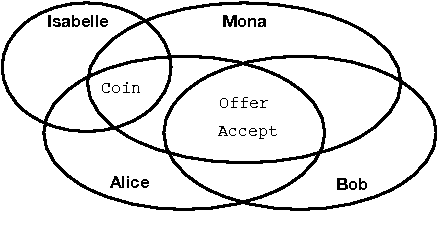
\includegraphics{figure/coin-transfer-visibility.pdf}
\end{center}
\vspace{-2ex}
\caption{Fact Visibility in Coin Transfer Example}
\label{f:CoinTransferVisibility}
\end{figure}

In many practical commercial workflows, it is either not desirable or not legal for all parties to be able to see all data in the system. In the coin transfer example from \S\ref{s:FactsWeights}, suppose that Alice wishes to transfer a coin to Bob, but does not want to reveal the total number of coins she holds. Recall from \S\ref{s:Observation} that a party can see a fact when it is listed in either its \emph{by-authority} set or its \emph{obs-authority} set. We can express this as a simple predicate, where the functions \trm{auth-by} and \trm{auth-obs} retrieve the respective metadata from a fact value.
$$
\trm{sees}~ P~ F = |(\trm{auth-by}~F \cup \trm{auth-obs}~F) \cap \{P\}| \ge 0
$$
Applying this predicate to the initial facts from \S\ref{s:NowWithMetadata} we see that we already have the desired situation. The coin fact and its weight is visible to Alice (the giver), and Mona (the monitor), while the Offer and Accept facts are visible to all three of Alice, Bob and Mona. Figure~\ref{f:CoinTransferVisibility} shows this in diagrammatic form.


% -----------------------------------------------------------------------------
\subsection{Transactions and Validation}
Maintaining fact privacy has implications for the underlying implementation. Assume that Alice, Bob and Mona all have their own computers in their own offices that each initially contain the subset of facts that each can see as per Figure~\ref{f:CoinTransferVisibility}. Assume that each party also has a copy of the transfer rule shown in Figure~\ref{f:CoinTransfer}. Now, suppose Alice decides that it is time to perform the transfer. On her own computer she executes the rule while recording the facts that have been consumed and the new facts that have been produced. She then builds a transaction data structure that records this information along with the cryptographic hash of the rule code, which we describe as so:

\begin{small}
\begin{code}
Transaction
{ ident = ... fresh number ...
, rule  = ... hash of code for transfer rule ...
, spent
   = [ Offer  [id = '1234, give = !Alice, recv = !Bob]
        by  {!Bob}              obs {!Mona, !Alice}
        use {'transfer}         num 1

     , Accept [id = '1234, acc = !Bob]
        by  {!Alice}            obs {!Mona, !Bob}
        use {'transfer}         num 1

     , Coin   [issuer = !Isabelle, holder = !Alice]
        by  {!Isabelle, !Alice} obs {!Mona}
        use {'transfer}         num 1 ]
, new
   = [ Coin   [issuer = !Isabelle, holder = !Bob]
        by  {!Isabelle, !Bob}   obs {!Mona}
        use {'transfer}         num 1 ]
\end{code}
\end{small}

This is the complete transaction that describes all inputs and outputs. For now, we will broadcast the entire transaction as to all parties in the network. In the next section we will discuss how to ensure that parties are only able to see the input and output facts that they are observers for.


% -----------------------------------------------------------------------------
\subsection{Blinded Transactions}
Alice can send the complete transaction to Mona, which is also entitled to see all the input and output facts, however we cannot also sent it to Isabelle and Bob because they are not entitled to see some of the components.

Instead, we can compute a \emph{restricted view} of the transaction for both Isabelle and Bob, which consists of a blinded hash of the entire transaction, along with a version of the transaction structure where the facts that a particular party are not entitled to see are replaced by blinded hashes of those facts. A \emph{blinded} hash is a regular cryptographic hash which has been combined with a salt value so that it cannot be easilly brute forced.

\TODO{In above transaction the meta-data reveals that it can be formally seen by Isabelle, Bob and Mona, though of course Alice knows about it as she built the transaction}. Distinguish between observer, formal observer, and incidental observer. As Alice is only an incidental observer she should not retain the fact data, as she will not receive information about transactions that spend this fact. Any transactions she might form based on this information may be invalid without her knowing.


For upgrade, the data model itself does not depend on hashing. In DAML contract ids are hashes that include the code of the template. In Rainfall hashing is used as part of the transaction structure but the fact that fact identity includes the hash of the rule that uses it does not leak into the programming model.


% -----------------------------------------------------------------------------
\subsection{Consistency}
\TODO{back ref to this from the related work section}
In Rainfall there is nothing stopping a party from adding a fact to the system which says ``I have a million dollars", just with their own authority. The key property we need to manage is whether anyone else should rightly believe them. Recall that in the coin transfer example from \S\ref{s:Facts}, the coin facts always carry the authority of multiple parties, which is justified by the sequence of transactions that result in their production. The coin issuer (@Isabelle@ in the example) initially creates, specifies the rules for using them, and signs the facts with their own authority. When the coins are transferred onwards the recorded transactions are also signed by the parties that propose them. Assuming most parties in the system are honest, invalid transactions will simply not be confirmed. Dishonest parties are free to corrupt their own databases by adding invalid transactions, but no one else using the system will accept them.






\clearpage{}
\section{Semantics}

% ---------------------------------------------------------
\begin{figure}
\begin{small}
\begin{alltt}
Name   ::= ...
Ctor   ::= ...
Label  ::= ...

Decl   ::= rule Name Rule
Rule   ::= await Guard+ to Action
Guard  ::= Ctor as Var where Term

Type   ::= unit | text | symbol | nat | party
        |  set Type | Type \(\to\) Type

Term   ::= Var | Term Term | \(\lambda\) Var : Type \(\to\) Term
        |  [ (Label = Term)* ] | Term . Label

Value  ::= Lit | \(\lambda\) Var : Type \(\to\) Term
        |  [ (Label = Value)* ]

Action ::= done | Action ; Action
        |  say Ctor [ (Label = Exp)* ]
           by  Term  use Term  for Term  obs Term
\end{alltt}
\end{small}

\caption{Core Language Grammar}
\end{figure}


% ---------------------------------------------------------
\begin{figure*}

$$
\begin{array}{cl}

% -- runs -----------------------------
\fbox{$\jRun{Auth}{Env}{Action}{Store}$}
\\[2ex]


% -- match ----------------------------
\fbox{$\jMatch{Auth}{Env}{Store}{Guard}{Auth}{Env}{Store}$}
\\[2ex]

% -- MatchGuard
\ruleI
{ \begin{array}{ll}
     E''   = E,~X\mapsto~\krecord~E'
  &  A \supseteq A_\iby \cup A_\iobs
  \\ S'' \ = S' [\ C~E'~A_{\iby}~A_{\iobs}~A_{\ifor}~M_{\iuse}~\mapsto~0 \ ]
  &  ~~ \jEval{\cdot}{M_\iuse~(\kauth~A)}{\ktrue}
  \\ S~~ \ = S' [\ C~E'~A_{\iby}~A_{\iobs}~A_{\ifor}~M_{\iuse}~\mapsto~1 \ ]
  &  \jEval{E''}{M}{\ktrue} \qq A' = A \cup A_\ifor
  \end{array}
}
{   \jMatch{A}{E}{S}{C~\kas~X~\kwhere~M}{A'}{E''}{S''}
}
& (\trm{Match})
\\[4ex]


% -- Matches ---------------------------
\fbox{$\jMatches{Auth}{Env}{Store}{Guard}{Auth}{Env}{Store}$}
\\[2ex]

% -- MatchNil
\ruleI
{ }
{\jMatches{A}{E}{S}{\cdot}{A}{E}{S}
}
& (\trm{MatchesNil})
\\[2ex]

% -- MatchCons
\ruleI
{   \jMatch  {A}{E}{S}{G}{A'}{E'}{S'}
\qq \jMatches{A'}{E'}{S'}{Gs}{A''}{E''}{S''}
}
{   \jMatches{A}{E}{S}{G,~Gs}{A''}{E''}{S''}}
& (\trm{MatchesCons})
\\[4ex]


% -- Fire -----------------------------
\fbox{$\jFire{Auth}{Store}{Decl}{Store}$}
\\[2ex]
\ruleI
{   \jMatches{A}{\cdot}{S}{G^n}{A'}{E'}{S'}
\qq \jRun{A'}{E'}{N}{S''}
}
{\jFire{A}{S}{\kawait~G^n~\kto~N}{S' \cup S''}
}
& (\trm{Fire})
\\[4ex]

\end{array}
$$

\caption{Operational Semantics}
\end{figure*}


\begin{figure}
\begin{small}
\begin{alltt}
fact  Coin   [stamp: Symbol, holder: Party]
fact  Offer  [id: Symbol, giver: Party, receiver: Party]
fact  Accept [id: Symbol, accepter: Party]

node  Bank

rule  transfer
await Accept  as accept
 and  Offer   as offer
      where   accept.id       == offer.id,
              accept.accepter == offer.receiver
 and  Coin    as coin
      where   coin.holder     == offer.giver
to
      say Coin [ stamp  = coin.stamp
               , holder = offer.receiver]
      by  [auth| Bank, offer.receiver]
      use (elem offer.receiver)

scenario Bank, Alice, Bob
to do say Coin   [ stamp = 'Coin1001, holder = Alice]
      by  [auth| Bank, Alice]
      use (elem Alice)

      say Offer  [ id    = '1234
                 , giver = Alice, receiver = Bob]
      by  Alice use (elem Bob)

      say Accept [ id = '1234,    accepter = Bob]
      by  Bob   use (const true)
\end{alltt}
\end{small}

\caption{Coin Transfer Workflow}
\label{f:CoinTransferDesugared}
\end{figure}



\label{s:Related}
\section{Related Work}

% ---------------------------------------------------------
\subsection{Linda-style Tuple Spaces}
Linda~\cite{Gelernter1985:Linda} is a coordination model where processes communicate by adding, removing and non-destructively reading tuples from a globally shared tuple space. The basic Linda model is open, meaning that any party using it is free to add and remove tuples at will. This lack of access control or provenance information makes it unusable for as a communication medium for mutually distrusting parties.

Several extensions to the basic Linda model add metadata to the tuples that are similar to the `by' and `obs' authority sets of our own Rainfall model. SecSpaces~\cite{Busi2003:SecSpaces} signs tuples with the private keys of parties that create them, and adds metadata that specifies the identities of those that can see and consume them. Merrick~\cite{Merrick2000:Scopes} describes a scoping/visibility system for tuple spaces where new scopes can be created at will and combined using a set of scope combinators. Oriol~\cite{Oriol2005:TaggedSets} describes a model of tagged sets where the tuples are identified by a formula in propositional logic that allows authority and visibility information to be encoded uniformly. Udzir~\cite{Udzir2007:MultiCapabilities}~describes a model where collections of tuples have unique identifiers, and the client program must provide a matching runtime capability when accessing them. These systems refine the Linda data model, but do not provide a mechanism to allow parties using the system to combine authorized tuples to produce new ones that are authorized by any other party except themselves. The ability to do this is the main contribution of our own system.


% ---------------------------------------------------------
\subsection{Law Governed Linda}
Law Governed Linda~(LGL)~\cite{Minsky1994:LawGovernedLinda, Minsky2001:SafeTupleSpace} takes the basic Linda data model and inserts a \emph{controller} between the tuple space and each communicating process. Each controller has a copy of a communication law, written in a fragment of Prolog, that specifies the allowable interactions with the tuple space. For example, the law could  state that a process may only create a tuple that includes a @from@ field, when the value in that field is its own process identifier.

The codified law specifies the allowable \emph{interaction} a process may have with the communication medium. The controllers are assumed to run on a trusted computing base, either as part of the physical server that provides the tuple space, or on a secure co-processor~\cite{Minsky2001:SafeTupleSpace}. In contrast, the production rules in our Rainfall model do not limit the form of data added to the system. Instead, they specify how authorized facts that are already in the store may be combined to produce new authorized facts. The Authority Flow theorem of \S\ref{s:PropertiesOfSemantics} also ensures we do not need to rely on a trusted computing base to enforce the rules of the system.


% ---------------------------------------------------------
\subsection{Extended Shared Prolog}
\label{s:RelatedESP}
Like LGL, Extended Shared Prolog (ESP)~\cite{Ciancarini1993:Coordinating, Ciancarini1994:LogicTupleSpaces} combines the Linda coordination model with rules written in a restricted subset of Prolog. In this case the rules are stored as special \emph{program tuples} in the main tuple space, and the rules describe how existing tuples can be combined, rather than controlling the interaction between the tuple space and its clients. The format of each rule is similar to a Rainfall production rule, including a section to gather matching tuples, a section to decide which should be consumed, and a section to compute new tuples. Program tuples behave like triggers in an active database~\cite{Paton1999:Active}, where a rule is activated when all tuples it was waiting for become available. However, as with the basic Linda coordination model, there is no mechanism to enforce transitive authority, or track the provenance of created tuples.

% Rainfall takes extends the basic ESP model with an authority mechanism to track which parties authorize the production of which facts, which allows the safe execution of multiparty contracts. ESP program rules are also anonymous, where the Rainfall system relies on them having names so that these names can be mentioned in the facts.

% Another minor difference is that the ESP fact matching system does not have direct support for aggregation operators as used in \REF. Aggregation is a key operation in regular database query languages, though usually not a primitive operation in Prolog style systems based around matching of Horn clauses. However, one can imagine support for aggregations being added via \emph{view tuples}, where the act of matching invokes an aggregation operation across some larger subset of the tuple space, as per LighTS~\cite{Balzarotti2007:LighTS}.


% ---------------------------------------------------------
\subsection{Permissioned Distributed Ledgers}
\label{s:RelatedPermissioned}
As mentioned in \S\ref{s:NestedTransactions}, DAML combines facts and rules into a \emph{contract instance}, which is similar to an object in an Object-Oriented (OO) model. Objects are referred to by \emph{contract identifiers}, which are equivalent to typed references in the OO model. The DAML coordination model is based on UTxO~\cite{Zahnentferner2018:UTxO}, so invoking a method on an object typically causes it to create some new objects, then consume/delete that object. Deleting an object causes any existing references to it to become dangling, and following a dangling reference at runtime causes an exception. In contrast, our Rainfall model identifies facts by their content, rather than using a physical reference or pointer value. If a particular fact is not available with sufficient weight then this inhibits rule firing, rather than being treated as an execution failure.

A DAML method can invoke methods on other objects that it already has a reference to, but cannot query the ledger state directly. This restriction is standard in the OO coordination model, where method code cannot directly query the runtime heap to discover other objects based on their field data. Instead, objects typically communicate using shared references to mutable data. However, as the DAML programming model purposefully does not include shared mutable data, the usual OO programming patterns are unavailable. In practice, ledger actions are performed by ``nanobots'', which are driver routines written in an external language. The query performed by a nanobot yields a set of contract identifiers, which are then passed back to the DAML code as arguments to method invocations. The Rainfall model was specifically developed to avoid the need for nanobots, while providing an authority system similar the one in DAML.

% Source level DAML programs could be converted to the Rainfall model by representing active DAML contract instances as facts listing their fields, and splitting each method into a separate rule. A party wishing to invoke a method would add a fact listing the arguments to that method, and the associated rule would consume both facts.

Corda~\cite{Hearn2016:Corda}, and Hyperledger Fabric~\cite{Androulaki2018:Fabric} are related permissioned distributed ledgers. Instead of defining a specific contract language, both systems allow custom procedures to be installed that accept transactions directly and report whether they are valid. In Corda the validation procedures are expressed in a version of JVM bytecode that has been modified to ensure execution is deterministic. In Hyperledger Fabric the validation procedures can be arbitrary native code encapsulated in a Docker~\cite{Docker2019} container. These systems both provide the networking layer for a distributed ledger system, but purposefully do not specify a programming model in sufficient detail to prove safety properties such as those in \S\ref{s:Properties}. Leaving this as a separate implementation design choice.


% ---------------------------------------------------------
\subsection{Actors, Process Algebras, and Constraints}
Production rule systems like Rainfall have a passing similarity to the Actor~\cite{Agha92:ActorTheory} model, but the computation framework is quite different. Production rules do not maintain their own private state, or have instance identity in the sense that they are addressable by mailbox or channel names. However, one could compile an actor program \emph{into} Rainfall, by building facts that represent the local state of each actor, and defining production rules to handle the messages. A proposed extension to Erlang provides the multi-headed pattern matching needed by production rules~\cite{Sulzmann2008:MultiHeaded}, though matching is performed on ordered streams of incoming messages, rather selecting from an unordered soup of tuples. ActorSpaces~\cite{Agha1993:ActorSpace} is a related model that uses message passing communication while also allowing messages to be broadcast to all actors in a group.

Existing process languages such as the Join Calculus~\cite{Cedric1996:Reflexive} and the Chemical Abstract Machine~(CHAM)~\cite{Berry1992:Chemical} allow processes to wait for multiple related facts (messages) to become available before activating. Similar functionality is available from of Constraint Handling Rules (CHR)~\cite{Fruthwirth1998:CHRs}. However, as with Extended Shared Prolog~(\S\ref{s:RelatedESP}) these systems do not have a builtin authority or provenance mechanism that could be used to guide data privacy as described in \S\ref{s:Privacy}.


% ---------------------------------------------------------
\subsection{Authorization Logics}
The Dependency Core Calculus (DCC)~\cite{Abadi1999:DCC} extends Moggi's computational lambda calculus with an extra judgment form that indicates the value produced by a computation is protected at a given security level. Abadi~\cite{Abadi2007:AccessControl} studies DCC applied to access control and tracking in a distributed system. This work uses a proposition $(P~\trm{says}~A)$, where $P$ is some principle/party that affirms statement $A$. The 'says' former abstracts away from the details of what exactly is being authenticated or authorized. The statement $(P~\trm{says}~A)$ can variously be interpreted as ``$P$ has caused $A$ to be said'', ``$A$ has been said on $P$'s behalf'' or ``$P$ supports $A$''. Garg~\cite{Garg2006:Constructive} gives a sequent style presentation with two judgement forms $(A~\trm{true})$ and $(P~\trm{affirms}~A)$. The `affirms' form is internalized as a proposition $(P~\trm{says}~A)$. Garg's system comes with meta theory of Affirmation Flow, meaning that unless a principle P affirms a particular statement, no affirmations of the form $(P~\trm{affirms}~A)$ can be derived from it. Bowers~\cite{Bowers2007:Consumable} gives a Gentzen style presentation that also has a $(P~\trm{signed}~A)$ form to model a message being cryptograpically signed.

DCC and related systems are logics rather than programming languages that have a direct operational interpretation. The Aura language~\cite{Jia2008:Aura} then specifies a functional operational semantics, as well as a proof term assignment for a version of DCC. Proofs of authority can be passed to functions as pure proof terms. Rainfall is directly inspired by the DCC family of logics and languages. Instead of building functional proof terms to demonstrate authority, we gather it in stages, incrementally writing authorized facts back to the ledger. Our ledger then can be viewed as a distributed proof of authority, where versions of DCC style logical properties still apply. For example, our Authority Flow theorem (\S\ref{s:Properties}) is the operational version of Garg's~\cite{Garg2006:Constructive} Affirmation Flow.

% -- cuts
% Rainfall rules have no breach state. Does not fit well into framework of Deontic or Defeasible logic, even though these are commonly used to describe contracts.



% Garg 2006~\cite{Garg2006:Constructive} presents a system in sequent style with two judgement forms (A true) and (K affirms A), where K is a principle (party) and A is a proposition. The 'affirms' judgement is then internalised into a proposition as (K says A). The meanings of the connectives are defined by the rules that introduce and eliminate them, rather than a concrete operationa semantics. This system comes with meta theory of affirmation flow, meaning that unless a principle K affirms a statement, no affirmations of the form (K affirms A) can be derived from it.

% Bowers 2007~\cite{Bowers2007:Consumable} contains a Gentzen style presentation of Garg 2006 that adds a linear environment to enforce that particular statements (K says A) are only used once in a given authority proof. It also has a (A signed F) form to model a message being cryptograpically signed. Includes an informal discussion of how linear uses of predicates can be enforced in a distributed environment by reling on a central ratifier to check the proofs.

% Aura~\cite{Jia2008:Aura} is a dependently typed language that includes the (A says P) form of DCC~\cite{Abadi1999:DCC} and provides a proof term assignment for the earlier pure authorization logics. The proof language is restricted to only contain proofs with no redexes, which simplifies type checking and ensures proof construction code does not perform effects. Proofs of authority are passed as pure proof terms so that fact that a given function may capture authority in its closure is not visible in its type.

% Rainfall system is not directly reactive, in the sense that there are concurrent processes waiting to receive messages and provide responses. As described in \REF, in normal use a submitting party decides when to perform a transaction according to one of the rules, and is free to disambiguate any non-determinism in pattern matching as they see fit.



% ---------------------------------------------------------
% \subsection{Production Engines}
% Our rules are closer to those used by production rule engines OPS~\cite{Forgy1981:OPS5} latter % versions CLIPS~\cite{Riley2017:CLIPS} and Drools~\cite{Proctor2008:Drools} do perform % non-deterministic matching. Implementations based on the RETE~\cite{Forgy1981:RETE} algorithm and % enhancements \cite{Doorenbos1995:ProductionMatching} of it. Our system is similar to a production % rule engine, but with the facts annotated by sets of parties and other authority metadata. In % systems like OPS the facts are part of a global set. In our system we annotate facts with sets of % parties that control visiblity.


% ---------------------------------------------------------
%\subsection{Account Based Ledgers}
% In public account ledgers like Ethereum~\cite{Wood2014:Ethereum} and EOS.IO~\cite{Lee2018:EOSIO} all data on the ledger is visible to all parties. In these systems each account is associated with a contract that has its own mutable state. The contract code can export methods which are callable by other parties in the system. Authority is managed programatically, where method code must check at runtime that the party that calls a particular method is permitted to do so. Contracts that require authority from multiple parties to perform some action can use local mutable state to build a set of parties that have provided their consent so far. In our system the authority to create and consume facts is managed at the meta level as this also affects the whether each party can see the data.

% Rules are free to perform their own ``business level'' checks, such as ensuring that only a given set of parties can activate the rule.


% ---------------------------------------------------------
% \subsection{Petri-net Systems}
% FCL~\cite{Adjoint2019:FCL} uses a petri net model with a baked in transaction system.
% Business Process Execution Language (BPEL)~\cite{Andrews2003:BPEL} itself lacks a formal semantics. Various efforts to assign semantics, eg using Petri Nets~\cite{Lohmann2009:PetriBPEL} and Abstract State Machines \cite{Fahland2005:SemanticsBPEL}. Much of the effort is in managing compensating transactions~\cite{Colombo2011:Compensating} which are a higher level language concern.


\textbf{Acknowledgements}
Many thanks to Fil Mackay, Lance Arlaus, Raphael Speyer, Erwin Ramirez and Ben Sinclair for helpful discussions and pointers to related work.


% -----------------------------------------------------------------------------
\clearpage{}
\bibliographystyle{plain}
\bibliography{Main}

% -----------------------------------------------------------------------------
\clearpage{}
\appendix
\section{Market example}

The market example introduced in~\S\ref{s:Selection} used the ``\trm{store-ok}'' invariant to ensure that, if the budgets are adhered to in a particular store, then after execution of any of the market rules, any updated budgets in the new store are also adhered to.
A budget is adhered to when the total value of invoices issued to a broker for a particular client do not exceed the client's specified budget limit.

\begin{tabbing}
M \= For all rules \= MMMMMM \kill
\> For all rules \> $r \in \{@accept@, @bid@, @reserve@\}$, \\
\> ~if   \> $\jFire{A_{sub}}{S}{r}{F_{read}^r}{D_{spent}^n}{D_{new}^m}{S'}$ \\
\> ~and \> $\trm{store-ok}~{S}$ \hspace{1ex} then \hspace{1ex} $\trm{store-ok}~{S'}$
\end{tabbing}

The definition of the invariant for stores finds all orders in the store, and ensures that for each order the order invariants are satisfied:

\begin{tabbing}
M \= M \= For all orders \= MMMMMM \kill
\> $\trm{store-ok}~{S} = $ \\
\> \> For all orders \> $@Order@~o \in S$, \\
\> \> require \> $\trm{order-ok}~{S}~o$
\end{tabbing}

The order invariant ensures that an order has at most one budget, and that the budget invariants are satisfied. An order with no associated budget is valid:

\begin{tabbing}
M \= M \= For all budgets \= MMMMMM \kill
\> $\trm{order-ok}~{S}~o = $ \\
\> \> For all budgets \> $@Budget@~b \in \trm{budgets-for-order}~S~o$, \\
\> \> require \> $\trm{unique}~S~b$ \\
\> \> and require \> $\trm{budget-ok}~{S}~b$
\end{tabbing}

While our desired property is to show that the total value of invoices does not exceed the budget limit, our invariant must show a stronger property, which is that the total value of bids, invoices and offers must not exceed the budget limit.
This stronger property is required as bids and offers can eventually result in invoices, as bids are transformed to offers, and offers are accepted. 
The budget invariant finds all associated bids, invoices and offers, and sums their prices to compute the total amount reserved by the budget. This total must not exceed the budget limit, and the remaining budget must be the difference between the total and the budget limit:

\begin{tabbing}
M \= M \= and require \= invoices \= \kill
\> $\trm{budget-ok}~{S}~b = $ \\
\> \> Require \> $\mathit{total} \le \trm{budget-total}~b$ \\
\> \> and require \> $\trm{budget-total}~b - \mathit{total} = \trm{budget-remain}~b$ \\
\> \> where \> $\mathit{total}$ \> $= \mathit{bids} + \mathit{invoices} + \mathit{offers}$, \\
\> \> and \> $\mathit{bids}$ \> $= \sum_{d \in \trm{bids-for-budget}~S~b} \trm{bid-price}~d$ \\
\> \> and \> $\mathit{invoices}$ \> $= \sum_{i \in \trm{invoices-for-budget}~S~b} \trm{invoice-price}~i$ \\
\> \> and \> $\mathit{offers}$ \> $= \sum_{o \in \trm{offers-for-budget}~S~b} \trm{offer-price}~o$ \\
\end{tabbing}

The functions \trm{bids-for-budget}, \trm{invoices-for-budget} and \trm{offers-for-budget} compute the multiset of associated bids, invoices or offers, for a particular budget. 
The functions \trm{budget-total}, \trm{budget-remain}, \trm{bid-price}, and so on, are accessor functions to retrieve components of the fact values.

\end{document}


